As mentioned above, tens of thousands of fibers need to be prepared and conditioned for the TRITIUM monitor\footnote{Tritium prototype will be a module of TRITIUM monitor, based on dozens of modules.}, section \ref{sec:TritiumMonitor}. Although this amount of fibers was not a problem for cutting, which is very fast, the polishing process is quite time consuming. It takes more than ten minutes to polish each fiber, that would result in an unaffordable amount of time to prepare the needed amount of fibers. Therefore, an automatic polishing machine for scintillating fibers was designed, built and tested. This polishing machine is able to polish up to one hundred scintillating fibers at the same time and automatically. Furthermore, it is easily scalable to larger capacity.

%\begin{figure}[htbp]
 %\centering
  %\subfloat[General view of Polishing machine.]{
   %\label{subfig:GeneralViewPolishingMachine}
    %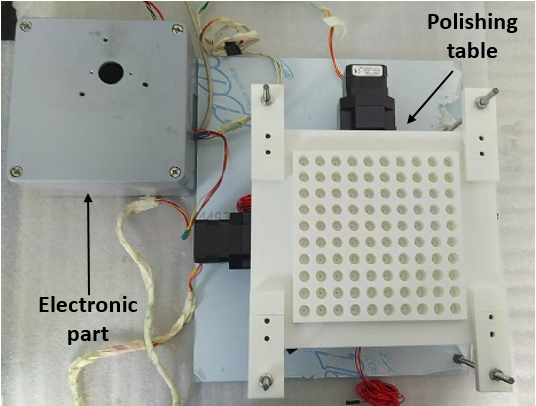
\includegraphics[angle=0, width=0.45\textwidth]{4ResearchAndDevelopments/41Fibers/GeneralViewPolishingMchine.png}}
    %\newline
  %\subfloat[Electronic system.]{
   %\label{subfig:ElectronicSystemPolishingMachine}
    %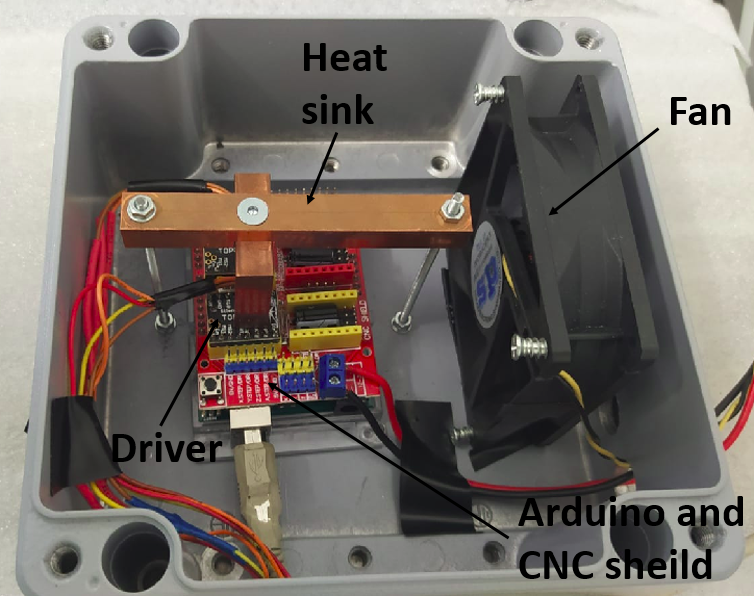
\includegraphics[angle=0, width=0.45\textwidth]{4ResearchAndDevelopments/41Fibers/ElectronicPolishingMachine.png}}
 %\caption{Polishing machine developed in TRITIUM experiment and the electronic system used.}
 %\label{fig:GeneralViewPolishingMachine}
%\end{figure}

\begin{figure}[h]
\centering
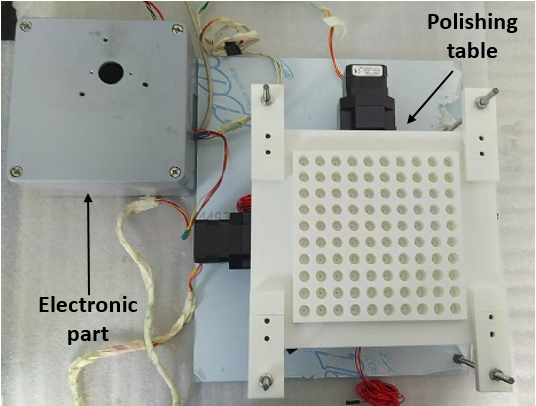
\includegraphics[scale=0.6]{4ResearchAndDevelopments/41Fibers/GeneralViewPolishingMchine.png}
\caption{Polishing machine developed in TRITIUM experiment.\label{fig:GeneralViewPolishingMachine}}
\end{figure}

This automatic polishing machine, displayed in Figure \ref{fig:GeneralViewPolishingMachine}, consists of two parts: 1) A polishing table, where the fibers are polished 2) The electronics, based on Arduino technology, that operates the movement of the polishing table:

\begin{enumerate}
\item{} The polishing table, shown in Figure \ref{subfig:PolishingTable}, is divided in two parts: the static part, where the fibers are fixed, and the movable part, where the polishing papers are fixed. It was decided to set the polishing papers on the movable part because they are lighter and less fragile than fibers.

The static part consists of a piece, shown in Figure \ref{subfig:PolishingTable},built with a 3D printer and fixed to the system by four vertical screws. On each screw there are two nuts to set the relative height and the inclination of fibers to the polishing papers. This piece contains one hundred holes in which the fibers are placed. 

The own weight of fibers press the polishing paper. As they are too light ($0.16~\gram$), a plastic belt and a piece of metal with a weight of around $1.5~\gram$, shown in Figure \ref{subfig:FiberMetailcPiece}, is employed to increase their weight (in the same way as in Thorlabs polishing process).

The movable part consists of a flat PMMA plate of $18 \times 18~\cm^2$ to which the polishing paper is attached. This part is locked to two horizontal screws, perpendicular to each other that are used to set its position in the XY plane (horizontal plane), as shown in Figure \ref{subfig:HorizontalAxis}.

The polishing system contains several switches,  mounted on a piece made by a 3D printer, shown in Figures \ref{subfig:PolishingTable}, \ref{subfig:HorizontalAxis} and \ref{subfig:3DSwitchPiece}, which are used to find the origin of coordinates when the system is reinitiated and to stop the movable part when the end of the path is reached. 

\begin{figure}
\centering
    \begin{subfigure}[b]{0.55\textwidth}
    \centering
    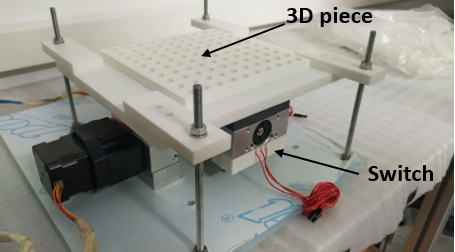
\includegraphics[width=\textwidth]{4ResearchAndDevelopments/41Fibers/PolishingTable.png}  
    \caption{Polishing table.\label{subfig:PolishingTable}}
    \end{subfigure}
    \hfill
    \begin{subfigure}[b]{0.3\textwidth}
    \centering
    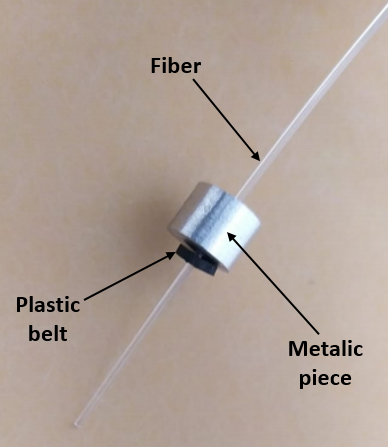
\includegraphics[width=\textwidth]{4ResearchAndDevelopments/41Fibers/PieceOfFiber.png}  
    \caption{Fiber with metal piece.\label{subfig:FiberMetailcPiece}}
    \end{subfigure}
    \hfill
    \begin{subfigure}[b]{0.55\textwidth}
    \centering
    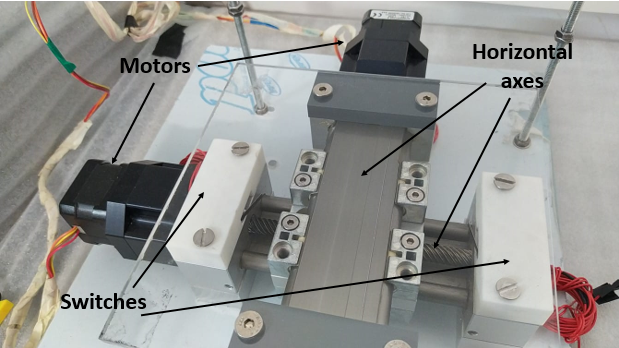
\includegraphics[width=\textwidth]{4ResearchAndDevelopments/41Fibers/HorizontalAxis2.png}  
    \caption{Horizontal screws and PMMA plate.\label{subfig:HorizontalAxis}}
    \end{subfigure}
    \hfill
    \begin{subfigure}[b]{0.4\textwidth}
    \centering
    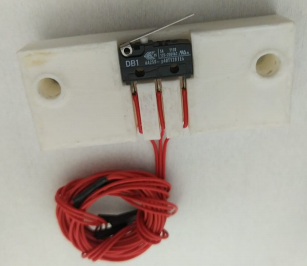
\includegraphics[width=\textwidth]{4ResearchAndDevelopments/41Fibers/Switch.png}  
    \caption{Piece to hold switches.\label{subfig:3DSwitchPiece}}
    \end{subfigure}
 \caption{Polishing table of the polishing machine}
 \label{fig:PolishingTable}
\end{figure}

\item{} The electronics, shown in Figure \ref{fig:ElectronicSystemPolishingMachine}, is based on Arduino technology which controls the automatic movement of the polishing paper.

The electronics consists of two stepper motors, model NEMA ST4209S1404-A \cite{StepperMotors}, which move the horizontal screws on which the polishing paper is attached. These motors are controlled by an Arduino UNO \cite{ArduinoUNO} that uses a CNC shield \cite{CNCShield} in which two different drivers are connected to control the stepper motors, one driver for each stepper motor.

Drivers are controllers that allow to manage stepper motors in a simple way. It is very important to choose the correct controller for the system because the controller limits the supply power to the motors, avoiding burning of the motors in the worst case. Instead of using the Pololu A4988 drivers \cite{A4988Driver}, which is one of the most widely used drivers, the first choice was the DRV8825 driver \cite{DRV8825Driver}. DRV8825 allows to power the motor with higher voltage and intensities ($45~\volt$ and $2.5~\ampere$) than A4988 ($35~\volt$ and $2~\ampere$). Also, the DRV8825 controller includes a new microstepping mode ($1/32$) compared to the A4988 ($1/16$) with which we get more accurate and smooth movements. Finally the drivers were replaced by the TMC2208 \cite{TMC2208Driver}, much less noisy since it includes the \textit{StealthChop} function with which the noise is practically eliminated. Furthermore, this controller is much more accurate as it has a microstepping mode of $1/256$. The voltage and current used to power the motors are $35~\volt$ and $2~\ampere$ which is sufficient for the whole system since the current of the motors is limited to $1.33~\ampere$. The excess current will be transformed into heat that has to be dissipated from the system. Overheating of the drivers may cause loss of steps, producing different movements from those programmed or even destroying the driver. Therefore, a cooling system is needed to ensure the correct operation of the polishing system. The cooling system, shown in Figure \ref{fig:ElectronicSystemPolishingMachine}, consists of a copper piece\footnote{The copper is one of the best thermal conductor at STP} in contact with both controllers and a fan, used to prevent heat accumulation inside the electronics box. The cooling power can be inproved by using a PELTIER cell.

\begin{figure}[h]
\centering
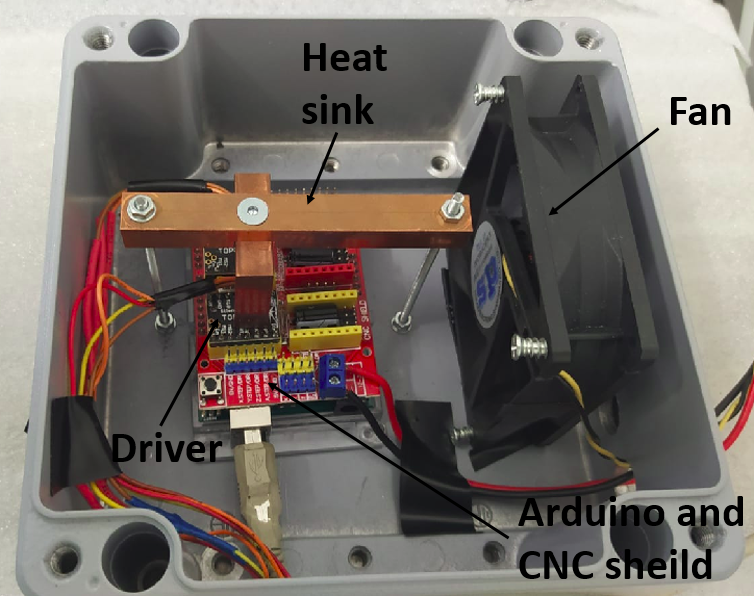
\includegraphics[scale=0.6]{4ResearchAndDevelopments/41Fibers/ElectronicPolishingMachine.png}
\caption{Electronic system of Polishing machine.\label{fig:ElectronicSystemPolishingMachine}}
\end{figure}

\end{enumerate}

This polishing machine is controlled by a computer using the Universal G-code Sender software (a grafical interface based on the GRBL package). There are several useful pre-programmed functions such as "HOME" with which the system, using the switches, finds its origin coordinate every time the system is turned on. 

The software also has the possibility of loading a file containing the g-code to be executed, In the TRITIUM, the 120 movements required for each polishing paper are loaded in this way. 

This machine was tested with twenty fibers of $15~\cm$ length arranged in a bundle. The fibers were fixed to the structure shown in Figure \ref{fig:BunchWith2PMTsCoincidence} and two PMTs located at the bundle ends, read in coincidence as described in section \ref{subsubsec:PMTsElectronicalSystem}, Figure \ref{subfig:ElectronicConfiguraiton2PMT}.

\begin{figure}[]
\centering
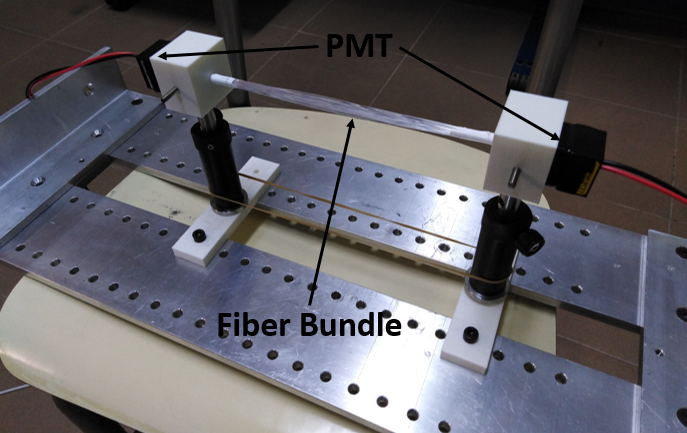
\includegraphics[scale=0.45]{4ResearchAndDevelopments/41Fibers/FiberBunch2PMTsCoincidence.png}
\caption{Set up used to test the effect of the polishing machine.\label{fig:BunchWith2PMTsCoincidence}}
\end{figure}

Two different measurements were taken using two different radioactive sources, a $\ce{^{60}Co}$ gamma source of $715~\becquerel$ activity, and a $\ce{^{90}Sr}$ beta source of $17.8~\kilo\becquerel$ activity. After, the fiber bundle was polished and the test was repeated.

The energy spectra recorded for both radioactive source are exhibited in Figure \ref{fig:ResultsOfPolishingMachine}. The sources were placed in the middle of the fiber bundle, at $7.5~\cm$ from each PMT.

\begin{figure}
\centering
    \begin{subfigure}[b]{0.76\textwidth}
    \centering
    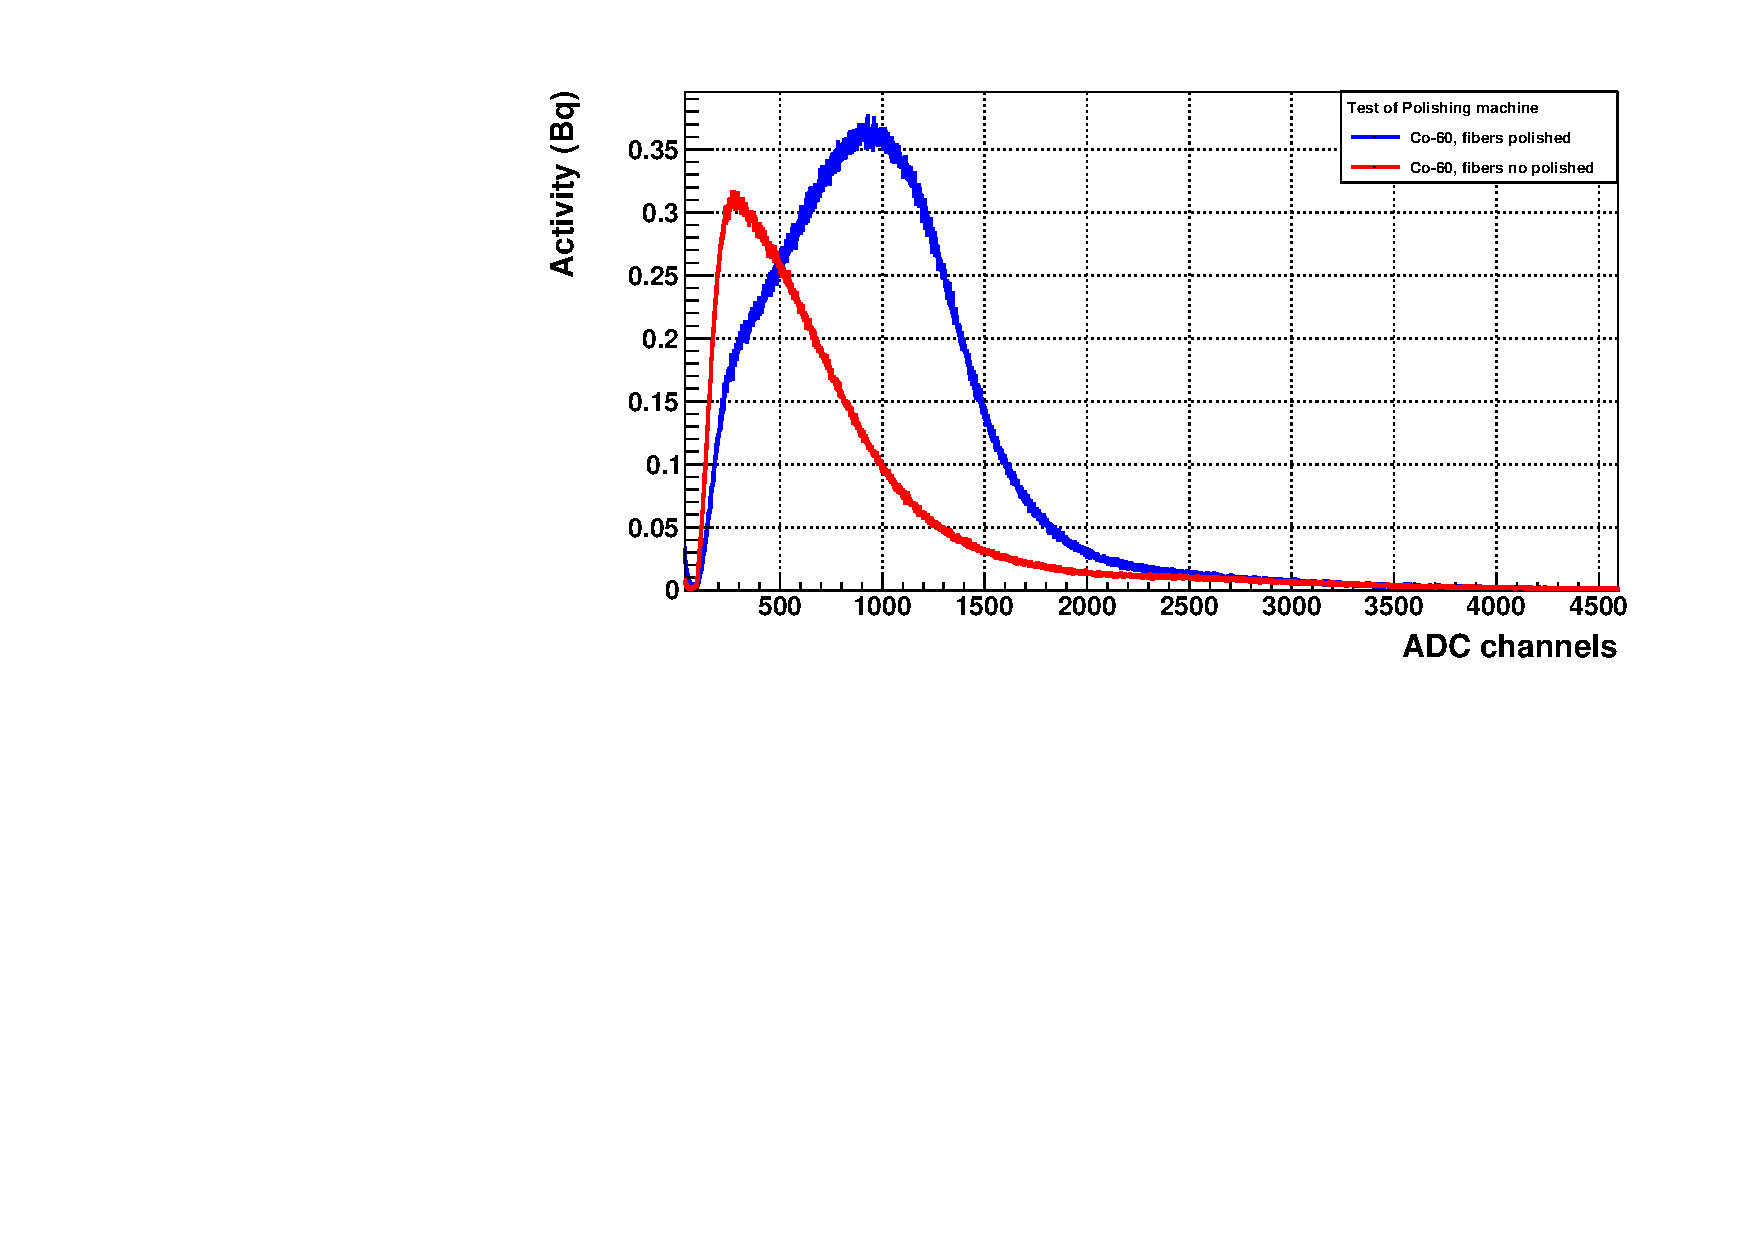
\includegraphics[width=\textwidth]{4ResearchAndDevelopments/41Fibers/Co_60_PolishingMachine_ZOOM.pdf}  
    \caption{Energy spectrum recorded for the Co-60 source.\label{subfig:EnergySpectrumCo60PolishingTest}}
    \end{subfigure}
    \hfill
    \begin{subfigure}[b]{0.76\textwidth}
    \centering
    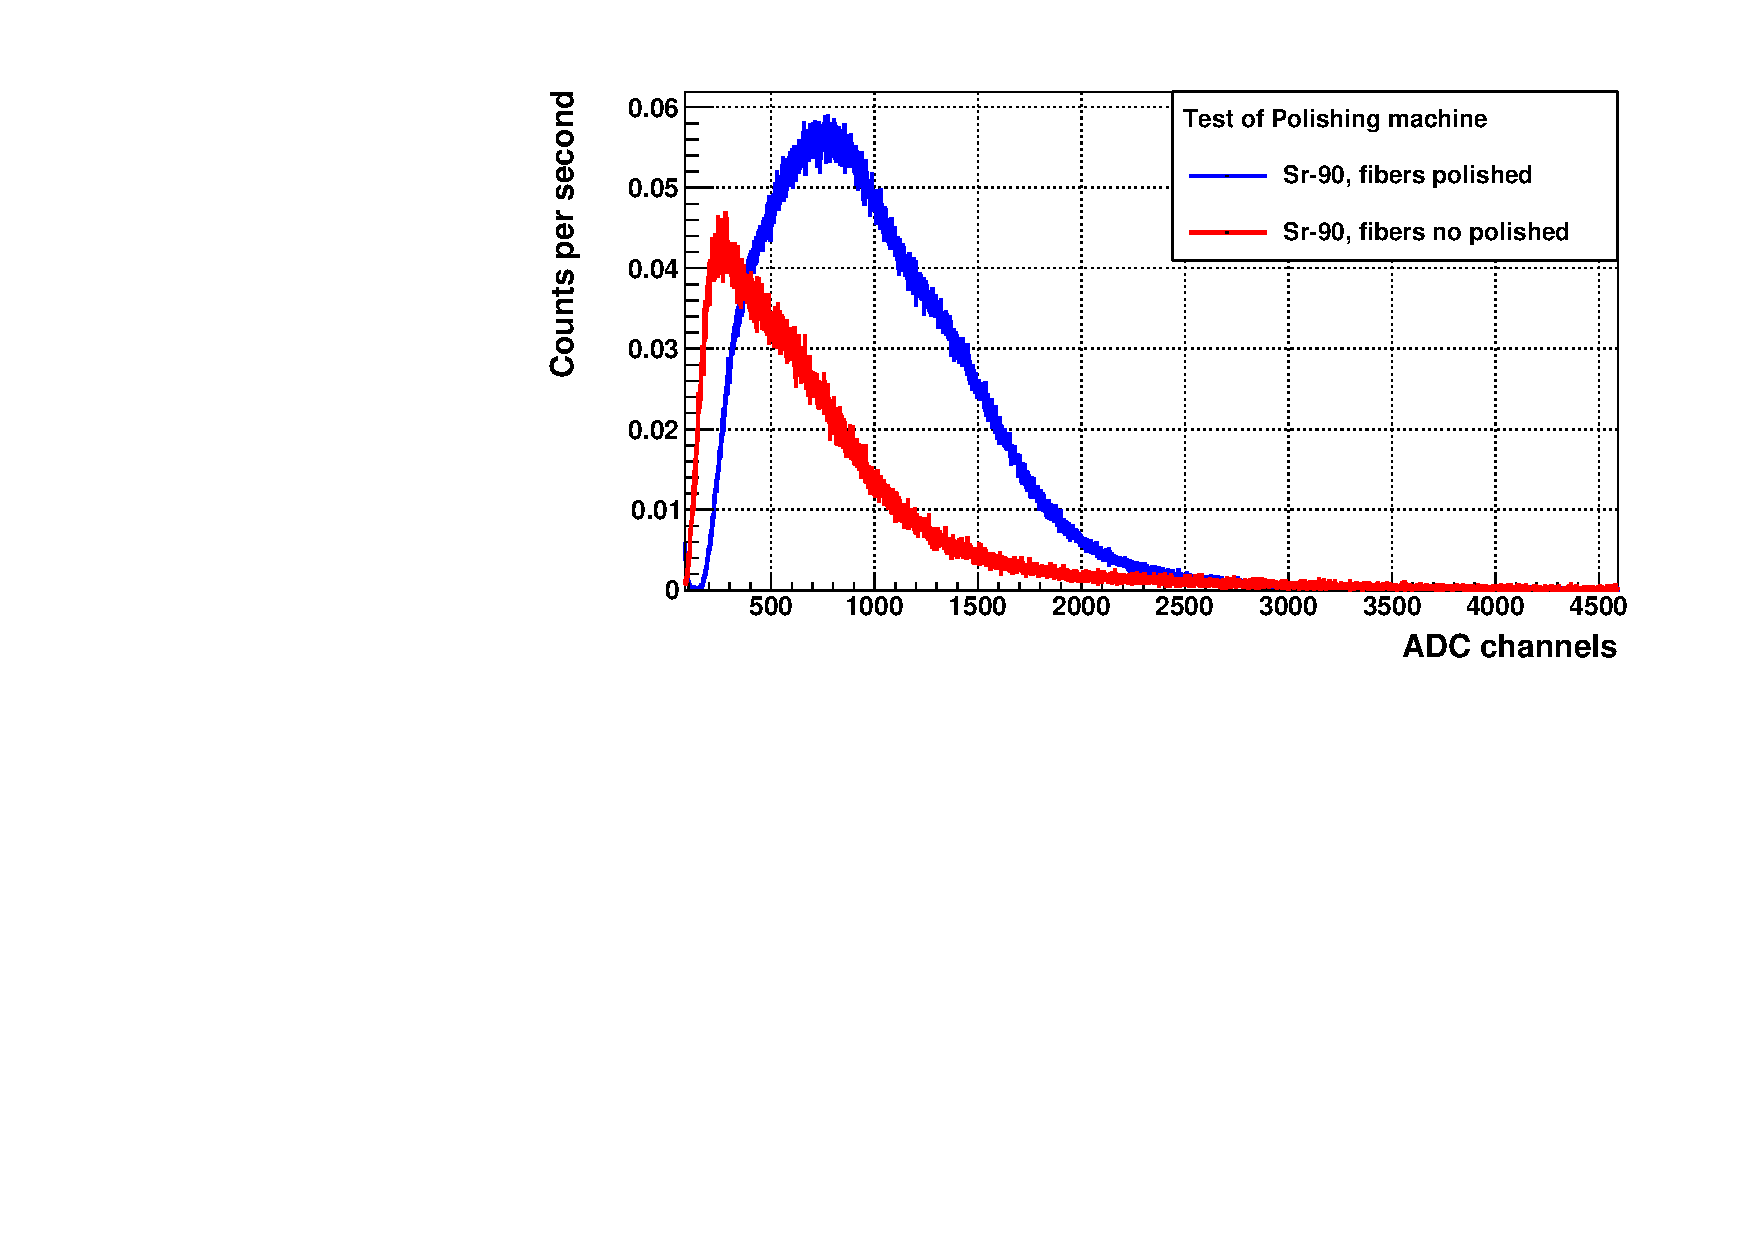
\includegraphics[width=\textwidth]{4ResearchAndDevelopments/41Fibers/Sr_90_PolishingMchine_ZOOM.pdf}  
    \caption{Energy spectrum recorded for the Sr-90 source.\label{subfig:EnergySpectrumSr90PolishingTest}}
    \end{subfigure}
 \caption{Energy spectrums used to test the effect of the Polishing machine}
 \label{fig:ResultsOfPolishingMachine}
\end{figure}

As it can be seen in Figure \ref{fig:ResultsOfPolishingMachine}, both energy spectra are shifted to the right after polishing fibers, which means that the detected events have more energy (more photons per event reach the PMTs). This energy increase was more than 40\% ($(42 \pm 4.6)\%$ for gamma source and $(49 \pm 8.4)\%$ for beta source) with respect the unpolished fiber. In summary, with the polishing machine, the photon collection efficiency of the fibers was improved  (mainly due to the improvement of the interface between fibers and PMTs). It is very important to achieve a high detection efficiency as the expected number of photons per tritium event is quite low.